\documentclass{ximera}
\graphicspath{  %% When looking for images,
{./}            %% look here first,
{./pictures/}   %% then look for a pictures folder,
{../pictures/}  %% which may be a directory up.
{../../pictures/}  %% which may be a directory up.
{../../../pictures/}  %% which may be a directory up.
{../../../../pictures/}  %% which may be a directory up.
}

\usepackage{listings}
\usepackage{circuitikz}
\usepackage{xcolor}
\usepackage{amsmath,amsthm}
\usepackage{subcaption}
\usepackage{graphicx}
\usepackage{tikz}
\usepackage{tikz-3dplot}
\usepackage{amsfonts}
\usepackage{mdframed} % For framing content
\usepackage{tikz-cd}

  \renewcommand{\vector}[1]{\left\langle #1\right\rangle}
  \newcommand{\arrowvec}[1]{{\overset{\rightharpoonup}{#1}}}
  \newcommand{\ro}{\texttt{R}}%% row operation
  \newcommand{\dotp}{\bullet}%% dot product
  \renewcommand{\l}{\ell}
  \let\defaultAnswerFormat\answerFormatBoxed
  \usetikzlibrary{calc,bending}
  \tikzset{>=stealth}
  




%make a maroon color
\definecolor{maroon}{RGB}{128,0,0}
%make a dark blue color
\definecolor{darkblue}{RGB}{0,0,139}
%define the color fourier0 to be the maroon color
\definecolor{fourier0}{RGB}{128,0,0}
%define the color fourier1 to be the dark blue color
\definecolor{fourier1}{RGB}{0,0,139}
%define the color fourier 1t to be the light blue color
\definecolor{fourier1t}{RGB}{173,216,230}
%define the color fourier2 to be the dark green color
\definecolor{fourier2}{RGB}{0,100,0}
%define teh color fourier2t to be the light green color
\definecolor{fourier2t}{RGB}{144,238,144}
%define the color fourier3 to be the dark purple color
\definecolor{fourier3}{RGB}{128,0,128}
%define the color fourier3t to be the light purple color
\definecolor{fourier3t}{RGB}{221,160,221}
%define the color fourier0t to be the red color
\definecolor{fourier0t}{RGB}{255,0,0}
%define the color fourier4 to be the orange color
\definecolor{fourier4}{RGB}{255,165,0}
%define the color fourier4t to be the darker orange color
\definecolor{fourier4t}{RGB}{255,215,0}
%define the color fourier5 to be the yellow color
\definecolor{fourier5}{RGB}{255,255,0}
%define the color fourier5t to be the darker yellow color
\definecolor{fourier5t}{RGB}{255,255,100}
%define the color fourier6 to be the green color
\definecolor{fourier6}{RGB}{0,128,0}
%define the color fourier6t to be the darker green color
\definecolor{fourier6t}{RGB}{0,255,0}

%New commands for this doc for errors in copying
\newcommand{\eigenvar}{\lambda}
%\newcommand{\vect}[1]{\mathbf{#1}}
\renewcommand{\th}{^{\text{th}}}
\newcommand{\st}{^{\text{st}}}
\newcommand{\nd}{^{\text{nd}}}
\newcommand{\rd}{^{\text{rd}}}
\newcommand{\paren}[1]{\left(#1\right)}
\newcommand{\abs}[1]{\left|#1\right|}
\newcommand{\R}{\mathbb{R}}
\newcommand{\C}{\mathbb{C}}
\newcommand{\Hilb}{\mathbb{H}}
\newcommand{\qq}[1]{\text{#1}}
\newcommand{\Z}{\mathbb{Z}}
\newcommand{\N}{\mathbb{N}}
\newcommand{\q}[1]{\text{``#1''}}
%\newcommand{\mat}[1]{\begin{bmatrix}#1\end{bmatrix}}
\newcommand{\rref}{\text{reduced row echelon form}}
\newcommand{\ef}{\text{echelon form}}
\newcommand{\ohm}{\Omega}
\newcommand{\volt}{\text{V}}
\newcommand{\amp}{\text{A}}
\newcommand{\Seq}{\textbf{Seq}}
\newcommand{\Poly}{\textbf{P}}
\renewcommand{\quad}{\text{    }}
\newcommand{\roweq}{\simeq}
\newcommand{\rowop}{\simeq}
\newcommand{\rowswap}{\leftrightarrow}
\newcommand{\Mat}{\textbf{M}}
\newcommand{\Func}{\textbf{Func}}
\newcommand{\Hw}{\textbf{Hamming weight}}
\newcommand{\Hd}{\textbf{Hamming distance}}
\newcommand{\rank}{\text{rank}}
\newcommand{\longvect}[1]{\overrightarrow{#1}}
% Define the circled command
\newcommand{\circled}[1]{%
  \tikz[baseline=(char.base)]{
    \node[shape=circle,draw,inner sep=2pt,red,fill=red!20,text=black] (char) {#1};}%
}

% Define custom command \strikeh that just puts red text on the 2nd argument
\newcommand{\strikeh}[2]{\textcolor{red}{#2}}

% Define custom command \strikev that just puts red text on the 2nd argument
\newcommand{\strikev}[2]{\textcolor{red}{#2}}

%more new commands for this doc for errors in copying
\newcommand{\SI}{\text{SI}}
\newcommand{\kg}{\text{kg}}
\newcommand{\m}{\text{m}}
\newcommand{\s}{\text{s}}
\newcommand{\norm}[1]{\left\|#1\right\|}
\newcommand{\col}{\text{col}}
\newcommand{\sspan}{\text{span}}
\newcommand{\proj}{\text{proj}}
\newcommand{\set}[1]{\left\{#1\right\}}
\newcommand{\degC}{^\circ\text{C}}
\newcommand{\centroid}[1]{\overline{#1}}
\newcommand{\dotprod}{\boldsymbol{\cdot}}
%\newcommand{\coord}[1]{\begin{bmatrix}#1\end{bmatrix}}
\newcommand{\iprod}[1]{\langle #1 \rangle}
\newcommand{\adjoint}{^{*}}
\newcommand{\conjugate}[1]{\overline{#1}}
\newcommand{\eigenvarA}{\lambda}
\newcommand{\eigenvarB}{\mu}
\newcommand{\orth}{\perp}
\newcommand{\bigbracket}[1]{\left[#1\right]}
\newcommand{\textiff}{\text{ if and only if }}
\newcommand{\adj}{\text{adj}}
\newcommand{\ijth}{\emph{ij}^\text{th}}
\newcommand{\minor}[2]{M_{#2}}
\newcommand{\cofactor}{\text{C}}
\newcommand{\shift}{\textbf{shift}}
\newcommand{\startmat}[1]{
  \left[\begin{array}{#1}
}
\newcommand{\stopmat}{\end{array}\right]}
%a command to give a name to explorations and hints and theorems
\newcommand{\name}[1]{\begin{centering}\textbf{#1}\end{centering}}
\newcommand{\vect}[1]{\vec{#1}}
\newcommand{\dfn}[1]{\textbf{#1}}
\newcommand{\transpose}{\mathsf{T}}
\newcommand{\mtlb}[2][black]{\texttt{\textcolor{#1}{#2}}}
\newcommand{\RR}{\mathbb{R}} % Real numbers
\newcommand{\id}{\text{id}}

\author{Zack Reed}
%borrowed from selinger linear algebra
\title{Inner Product Spaces and applications: PCA}
\begin{document}
\begin{abstract}

    One application of IPSs is PCA.

\end{abstract}
\maketitle


\section{Application: Principal component analysis}

%\begin{outcome}
%  \begin{enumerate}
%  \item Compute the principal components of a matrix $A$.
%  \item Compute the centroid of a collection of data points.
%  \item Find the $k$-dimensional subspace that best approximates a
%    given collection of data points.
%  \item Find the $k$-dimensional affine subspace that best
%    approximates a given collection of data points.
%  \item Compute the total squared distance of the data points to the
%    best fit subspace (or best fit affine subspace).
%  \end{enumerate}
%\end{outcome}

In this section, we will explore an application of the diagonalization
of symmetric matrices called \textbf{principal component analysis}.
Imagine we are given a collection of data points such as the
following:
\begin{equation}\label{eqn:subspace-fitting}
  \begin{tikzpicture}[baseline=-0.5ex]
    \draw[thin,->] (-4,0) -- (4,0);
    \draw[thin,->] (0,-4) -- (0,4);
    % \draw[thick,blue] (-4,-4/1.29) -- (4,4/1.29);
    \fill[color=red] (-2.25,-1.21) circle (0.06);
    \fill[color=red] (-1.44,-1.28) circle (0.06);
    \fill[color=red] (2.29,1.82) circle (0.06);
    \fill[color=red] (0.25,0.43) circle (0.06);
    \fill[color=red] (-1.57,-1.07) circle (0.06);
    \fill[color=red] (2.51,2.00) circle (0.06);
    \fill[color=red] (-2.53,-2.34) circle (0.06);
    \fill[color=red] (-3.04,-2.40) circle (0.06);
    \fill[color=red] (0.84,0.36) circle (0.06);
    \fill[color=red] (-3.16,-2.73) circle (0.06);
    \fill[color=red] (-2.02,-1.88) circle (0.06);
    \fill[color=red] (3.06,2.44) circle (0.06);
    \fill[color=red] (-1.40,-1.12) circle (0.06);
    \fill[color=red] (-2.09,-1.34) circle (0.06);
    \fill[color=red] (-1.23,-1.13) circle (0.06);
    \fill[color=red] (0.48,0.06) circle (0.06);
    \fill[color=red] (-1.49,-1.20) circle (0.06);
    \fill[color=red] (0.98,0.75) circle (0.06);
    \fill[color=red] (1.40,0.89) circle (0.06);
    \fill[color=red] (-0.12,0.09) circle (0.06);
    \fill[color=red] (0.88,0.40) circle (0.06);
    \fill[color=red] (-0.38,0.55) circle (0.06);
    \fill[color=red] (0.34,0.46) circle (0.06);
    \fill[color=red] (0.45,0.21) circle (0.06);
    \fill[color=red] (-0.59,-0.63) circle (0.06);
    \fill[color=red] (-0.53,-0.29) circle (0.06);
    \fill[color=red] (2.10,1.35) circle (0.06);
    \fill[color=red] (1.65,1.60) circle (0.06);
    \fill[color=red] (-3.88,-2.83) circle (0.06);
    \fill[color=red] (-0.07,-0.01) circle (0.06);
    \fill[color=red] (-0.37,-0.57) circle (0.06);
    \fill[color=red] (-0.99,-0.75) circle (0.06);
    \fill[color=red] (-2.34,-2.08) circle (0.06);
    \fill[color=red] (3.63,3.15) circle (0.06);
    \fill[color=red] (1.37,0.48) circle (0.06);
    \fill[color=red] (-0.96,-0.74) circle (0.06);
    \fill[color=red] (3.51,2.79) circle (0.06);
    \fill[color=red] (-3.33,-2.72) circle (0.06);
    \fill[color=red] (0.39,0.09) circle (0.06);
    \fill[color=red] (-1.38,-1.17) circle (0.06);
    \fill[color=red] (-0.36,-0.65) circle (0.06);
    \fill[color=red] (1.38,0.66) circle (0.06);
    \fill[color=red] (1.85,1.24) circle (0.06);
    \fill[color=red] (2.35,1.85) circle (0.06);
    \fill[color=red] (0.85,0.25) circle (0.06);
    \fill[color=red] (-0.23,0.19) circle (0.06);
    \fill[color=red] (-0.90,-0.74) circle (0.06);
    \fill[color=red] (2.50,1.31) circle (0.06);
    \fill[color=red] (-0.45,-0.71) circle (0.06);
    \fill[color=red] (0.92,0.56) circle (0.06);
    \fill[color=red] (0.97,1.21) circle (0.06);
    \fill[color=red] (-0.85,-0.74) circle (0.06);
    \fill[color=red] (-0.10,0.13) circle (0.06);
    \fill[color=red] (0.32,0.49) circle (0.06);
    \fill[color=red] (2.58,1.57) circle (0.06);
    \fill[color=red] (-0.59,-0.48) circle (0.06);
    \fill[color=red] (2.28,1.50) circle (0.06);
    \fill[color=red] (1.21,0.94) circle (0.06);
    \fill[color=red] (-0.35,-0.13) circle (0.06);
    \fill[color=red] (-1.53,-1.26) circle (0.06);
    \fill[color=red] (-2.77,-2.14) circle (0.06);
    \fill[color=red] (1.23,1.02) circle (0.06);
    \fill[color=red] (2.61,1.88) circle (0.06);
    \fill[color=red] (-0.04,-0.05) circle (0.06);
    \fill[color=red] (2.09,1.30) circle (0.06);
    \fill[color=red] (2.37,1.52) circle (0.06);
    \fill[color=red] (-2.01,-1.69) circle (0.06);
    \fill[color=red] (0.48,0.72) circle (0.06);
    \fill[color=red] (0.23,0.49) circle (0.06);
    \fill[color=red] (-1.16,-0.95) circle (0.06);
    \fill[color=red] (-0.14,-0.18) circle (0.06);
    \fill[color=red] (-1.57,-1.68) circle (0.06);
    \fill[color=red] (0.39,0.15) circle (0.06);
    \fill[color=red] (-0.24,-0.29) circle (0.06);
  \end{tikzpicture}
\end{equation}
Although these points are spread out in two dimensions, they seem to
be located pretty close to a 1-dimensional subspace. Probably the best
way to interpret this particular data set is to think of the points as
being ``essentially'' on a line, up to some small random errors.

More generally, suppose we are given a collection of data points in
$n$-dimensional space, and we are looking for a $k$-dimensional
subspace that all data points are close to.  This is an important way
to make sense of high-dimensional data. For example, it would be very
difficult to visualize data in a $100$-dimensional space. However, it
we knew that the data points lie very close to a 2-dimensional
subspace, then we could project all of the points to the subspace to
obtain a 2-dimensional image of the data.

To state the problem more precisely, let us introduce the following
notation. If $W$ is a subspace of $\R^n$ and $\vect{v}\in\R^n$ is a
vector, let us write $d(\vect{v},W)$ for the shortest distance from
$\vect{v}$ to $W$ (i.e., the distance from $\vect{v}$ to $W$ along a
line that is perpendicular to $W$). Moreover, if $W$ is a subspace of
$\R^n$ and $\vect{v}_1,\ldots,\vect{v}_m\in\R^n$ are the position
vectors of $m$ points, we define the \textbf{total squared distance}%
\index{distance!total squared distance}%
\index{squared distance}%
\index{total squared distance}%
\index{subspace fitting!total squared distance} of the points to
the subspace to be the quantity
\begin{equation*}
  D = d(\vect{v}_1,W)^2 + \ldots + d(\vect{v}_m,W)^2.
\end{equation*}
Then the problem we would like to solve can be stated as follows:

\begin{problem}{Subspace fitting problem}{subspace-fitting}
  Given vectors $\vect{v}_1,\ldots,\vect{v}_m\in\R^n$ and given an
  integer $k\leq n$, find the $k$-dimensional subspace
  $W\subseteq\R^n$ that minimizes the total squared distance, i.e.,
  such that $D$ is as small as possible%
  \index{subspace fitting}%
  \index{fitting!subspace fitting}.
\end{problem}

The following proposition gives us a method for solving the subspace
fitting problem. It turns out that the key ingredient in solving this
problem is the diagonalization of symmetric matrices. The method was
discovered by Gale Young%
\index{Young, Gale}%
\index{Gale Young} in 1937.

\begin{proposition}{Solution of the subspace fitting problem}{subspace-fitting}
  Given vectors $\vect{v}_1,\ldots,\vect{v}_m\in\R^n$ and $k\leq n$,
  the optimal solution to the subspace fitting problem can be computed
  as follows:
  \begin{enumerate}
  \item Let $A$ be the $m\times n$-matrix whose rows are
    $\vect{v}_1^T,\ldots,\vect{v}_m^T$. (Or equivalently, $A^T$ is the
    $n\times m$-matrix whose columns are
    $\vect{v}_1,\ldots,\vect{v}_m$.)
  \item Let $B=A^TA$. Then $B$ is a positive semidefinite
    $n\times n$-matrix.
  \item By Proposition~\ref{prop:characterize-positive}, all
    eigenvalues of $B$ are real and non-negative. Let
    $\eigenvar_1,\ldots,\eigenvar_n$ be the eigenvalues of $B$, listed
    according to their multiplicity and in decreasing order, i.e., so
    that $\eigenvar_1\geq\eigenvar_2\geq\ldots\geq\eigenvar_n\geq
    0$. Let $\vect{u}_1,\ldots,\vect{u}_n$ be the corresponding
    eigenvectors.
  \item Then $W=\sspan\set{\vect{u}_1,\ldots,\vect{u}_k}$ is the
    solution to the subspace fitting problem.  Moreover, the total
    squared distance of the points to this subspace is
    \begin{equation*}
      D = \eigenvar_{k+1} + \ldots + \eigenvar_n.
    \end{equation*}
  \end{enumerate}
\end{proposition}

\begin{example}{Subspace fitting in $\R^2$}{subspace-fitting-r2}
  Consider the following collection of points in $\R^2$:
  \begin{equation*}
    \set{
      \startmat{r}  2 \\ -3 \stopmat,
      \startmat{r} -1 \\  0 \stopmat,
      \startmat{r}  2 \\  3 \stopmat,
      \startmat{r} -6 \\ -7 \stopmat,
      \startmat{r}  6 \\ 11 \stopmat,
      \startmat{r}  0 \\ -1 \stopmat,
      \startmat{r}  1 \\  6 \stopmat,
      \startmat{r} -2 \\ -3 \stopmat,
      \startmat{r} -7 \\ -6 \stopmat
    }.
  \end{equation*}
  Find the 1-dimensional subspace that best approximates this
  collection of points. What is the total squared distance of the
  points to the subspace?
\end{example}

\begin{solution}
  We follow the steps outlined in
  Proposition~\ref{prop:subspace-fitting}.
  \begin{enumerate}
  \item We have
    \begin{equation*}
      A^T = \startmat{rrrrrrrrr}
        2 & -1 & 2 & -6 & 6 & 0 & 1 & -2 & -7 \\
        -3 & 0 & 3 & -7 & 11 & -1 & 6 & -3 & -6
      \stopmat.
    \end{equation*}
  \item We calculate
    \begin{equation*}
      B = A^TA = \startmat{rr}
        135 & 162 \\
        162 & 270
      \stopmat.
    \end{equation*}
  \item The eigenvalues of $B$ are $\eigenvar_1 = 378$ and
    $\eigenvar_2 = 27$, with corresponding eigenvectors
    \begin{equation*}
      \vect{u}_1 = \startmat{r} 2 \\ 3 \stopmat
      \quad\mbox{and}\quad
      \vect{u}_2 = \startmat{r} 3 \\ -2 \stopmat.
    \end{equation*}
  \item The desired subspace $W$ is spanned by the eigenvector
    corresponding to the largest eigenvalue, i.e.,
    $W=\sspan\set{\vect{u}_1}$. The total squared distance is
    $\eigenvar_2 = 27$.
  \end{enumerate}
  The space $W$ is shown in the following illustration, along with the
  original points:
  \begin{equation*}
    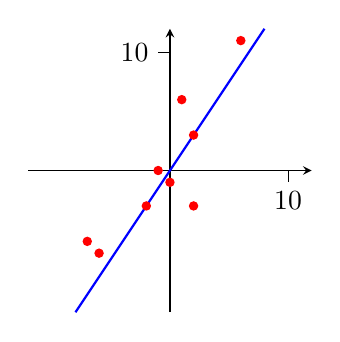
\begin{tikzpicture}[scale=0.15]
      \draw[thin,->] (-12,0) -- (12,0);
      \draw[thin,->] (0,-12) -- (0,12);
      \draw[thin] (0,10) -- (-1,10) node[left] {$10$};
      \draw[thin] (10,0) -- (10,-1) node[below] {$10$};
      \draw[thick,blue] (-8,-12) -- (8,12);
      \fill[color=red] (2,-3) circle (0.4);
      \fill[color=red] (-1, 0) circle (0.4);
      \fill[color=red] (2, 3) circle (0.4);
      \fill[color=red] (-6, -7) circle (0.4);
      \fill[color=red] (6, 11) circle (0.4);
      \fill[color=red] (0, -1) circle (0.4);
      \fill[color=red] (1, 6) circle (0.4);
      \fill[color=red] (-2, -3) circle (0.4);
      \fill[color=red] (-7, -6) circle (0.4);
    \end{tikzpicture}
  \end{equation*}
  Of course, the example was rigged to ensure that the eigenvalues are
  integers. In real life, the entries of $A$ and $B$, as well as the
  eigenvalues and components of the eigenvectors are usually arbitrary
  real numbers.
\end{solution}

\begin{example}{Subspace fitting in $\R^3$}{subspace-fitting-r3}
  Consider the following collection of points in $\R^3$:
  \begin{equation*}
    \set{
      \startmat{r} -7 \\ 4 \\ 5 \stopmat,
      \startmat{r} 0 \\ 3 \\ 3 \stopmat,
      \startmat{r} 2 \\ -5 \\ -4 \stopmat,
      \startmat{r} 10 \\ -4 \\ 1 \stopmat,
      \startmat{r} -2 \\ 5 \\ 4 \stopmat,
      \startmat{r} -8 \\ -1 \\ -5 \stopmat,
      \startmat{r} 5 \\ 4 \\ 2 \stopmat,
      \startmat{r} -6 \\ 9 \\ 6 \stopmat,
      \startmat{r} 9 \\ -6 \\ 3 \stopmat,
      \startmat{r} -2 \\ -7 \\ -8 \stopmat
    }.
  \end{equation*}
  %\begin{enumialphparenastyle}
    \begin{enumerate}
    \item Find the 1-dimensional subspace that best approximates this
      collection of points.
    \item Find the 2-dimensional subspace that best approximates this
      collection of points.
    \item What is the 3-dimensional subspace that best approximates this
      collection of points?
    \end{enumerate}
  %\end{enumialphparenastyle}
  In each case, what is the total squared distance of the points to
  the subspace?
\end{example}

\begin{solution}
  Again, we follow the steps from
  Proposition~\ref{prop:subspace-fitting}. We can do the calculations
  for parts (a), (b), and (c) at the same time.
  \begin{enumerate}
  \item We have
    \begin{equation*}
      A^T = \startmat{rrrrrrrrrr}
        -7 & 0 & 2 & 10 & -2 & -8 & 5 & -6 & 9 & -2 \\
        4 & 3 & -5 & -4 & 5 & -1 & 4 & 9 & -6 & -7 \\
        5 & 3 & -4 & 1 & 4 & -5 & 2 & 6 & 3 & -8 \\
      \stopmat.
    \end{equation*}
  \item We calculate
    \begin{equation*}
      B = A^TA = \startmat{rrr}
        367 & -154 & 16 \\
        -154 & 274 & 170 \\
        16 & 170 & 205 \\
      \stopmat.
    \end{equation*}
  \item The eigenvalues of $B$ are $\eigenvar_1 = 513$,
    $\eigenvar_2 = 306$, and $\eigenvar_3 = 27$, with corresponding
    eigenvectors
    \begin{equation*}
      \vect{u}_1 = \startmat{r} -2 \\ 2 \\ 1 \stopmat,
      \quad
      \vect{u}_2 = \startmat{r} 2 \\ 1 \\ 2 \stopmat
      \quad\mbox{and}\quad
      \vect{u}_3 = \startmat{r} -1 \\ -2 \\ 2 \stopmat.
    \end{equation*}
  \end{enumerate}

  For part (a), the desired 1-dimensional subspace is spanned by the
  eigenvector corresponding to the largest eigenvalue, i.e., it is
  $\sspan\set{\vect{u}_1}$. The total squared distance is
  $\eigenvar_2+\eigenvar_3 = 306 + 27 = 333$.

  For part (b), the desired 2-dimensional subspace is spanned by the
  eigenvectors corresponding to the two largest eigenvalues, i.e., it
  is $\sspan\set{\vect{u}_1,\vect{u}_2}$. The total squared distance is
  $\eigenvar_3 = 27$.

  Finally, in part (c), the desired 3-dimensional subspace is spanned
  by all three eigenvectors; it is of course $\R^3$ itself, since it
  is the only 3-dimensional subspace. The total squared distance is
  $0$, since all points lie in the subspace.
\end{solution}

The vectors $\vect{u}_1,\ldots,\vect{u}_n$ that appear in the solution
of the subspace fitting problem are called the \textbf{principal
  components} of the matrix $A$.

\begin{definition}{Principal components}{principal-components}
  Let $A$ be an $m\times n$-matrix. The \textbf{principal components}%
  \index{principal component}%
  \index{component!principal component} of $A$ are the (normalized,
  orthogonal) eigenvectors $\vect{u}_1,\ldots,\vect{u}_n$ of the
  positive semidefinite $n\times n$-matrix $A^TA$. They are usually
  listed in order of decreasing eigenvalues.
\end{definition}

The first principal component $\vect{u}_1$ gives the direction in
which the rows of $A$ show the most variability. The second principal
component $\vect{u}_2$ gives the direction in which the rows of $A$
show the most remaining variability that is orthogonal to
$\vect{u}_1$. The third principal component $\vect{u}_3$ gives the
direction of most variability that is orthogonal to $\vect{u}_1$ and
$\vect{u}_2$, and so on.

% ----------------------------------------------------------------------
\subsection*{Subspace fitting vs. curve fitting}

In the particular case where $n=2$ and $k=1$, we are looking for a
1-dimensional subspace, i.e., a line through the origin, which best
fits the given 2-dimensional data, as in the illustration
{\eqref{eqn:subspace-fitting}} above or as in
Example~\ref{exa:subspace-fitting-r2}. On its face, the subspace
fitting problem in this case seems similar to the linear curve
fitting%
\index{curve fitting} problem we solved in
Section~\ref{sec:least-squares}. However, there is a subtle but
important difference: in linear curve fitting, we were seeking to
minimize the distances of the points from the line in the
$y$-direction, whereas in subspace fitting, we are seeking to minimize
the distances of the points from the subspace in the direction
perpendicular to the subspace. The following pair of pictures
illustrates the difference:
\begin{equation*}
  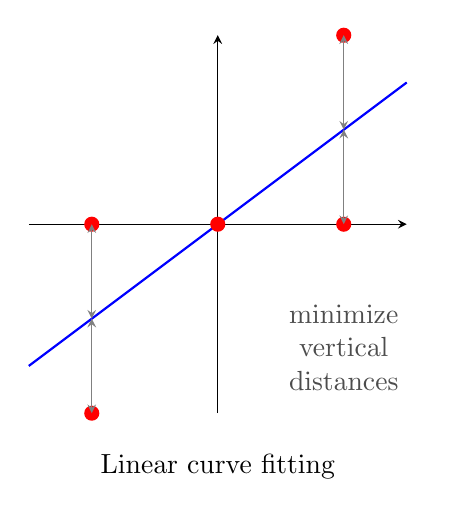
\begin{tikzpicture}[scale=0.8]
    \draw[thin,->] (-3,0) -- (3,0);
    \draw[thin,->] (0,-3) -- (0,3);
    \draw[thick,blue] (-3,-3*0.75) -- (3,3*0.75);
    \fill[color=red] (0,0) circle (0.12);
    \fill[color=red] (2,0) circle (0.12);
    \fill[color=red] (2,3) circle (0.12);
    \fill[color=red] (-2,0) circle (0.12);
    \fill[color=red] (-2,-3) circle (0.12);
    \draw[<->,black!50] (2,0) -- (2,1.5);
    \draw[<->,black!50] (2,3) -- (2,1.5);
    \draw[<->,black!50] (-2,0) -- (-2,-1.5);
    \draw[<->,black!50] (-2,-3) -- (-2,-1.5);
    \path (0,-3.5) node[below] {Linear curve fitting};
    \path[black!70] (2,-2) node {\begin{tabular}{c}minimize\\vertical\\distances\end{tabular}};
  \end{tikzpicture}
  \hspace{1in}
  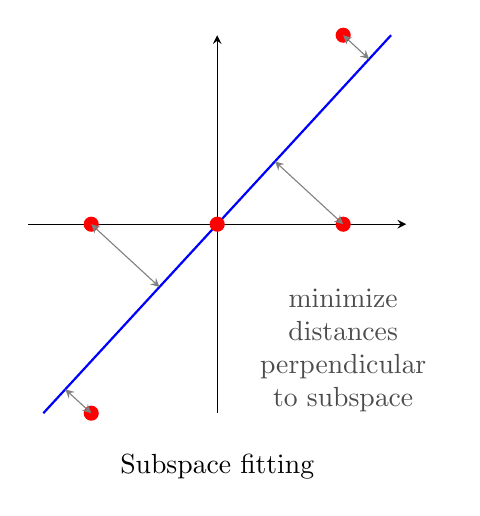
\begin{tikzpicture}[scale=0.8]
    \draw[thin,->] (-3,0) -- (3,0);
    \draw[thin,->] (0,-3) -- (0,3);
    \draw[thick,blue] (-3*0.92,-3) -- (3*0.92, 3);
    \fill[color=red] (0,0) circle (0.12);
    \fill[color=red] (2,0) circle (0.12);
    \fill[color=red] (2,3) circle (0.12);
    \fill[color=red] (-2,0) circle (0.12);
    \fill[color=red] (-2,-3) circle (0.12);
    \draw[<->,black!50] (2,0) -- (0.997*0.92,0.997);
    \draw[<->,black!50] (2,3) -- (2.621*0.92,2.621);
    \draw[<->,black!50] (-2,0) -- (-0.997*0.92,-0.997);
    \draw[<->,black!50] (-2,-3) -- (-2.621*0.92,-2.621);
    \path (0,-3.5) node[below] {Subspace fitting};
    \path[black!70] (2,-2) node {\begin{tabular}{c}minimize\\distances\\perpendicular\\to subspace\end{tabular}};
  \end{tikzpicture}
\end{equation*}

% ----------------------------------------------------------------------
\subsection*{Affine fitting}

So far, we have been looking to approximate a given collection of
points by a {\em subspace}, which necessarily passes through the
origin. But sometimes the points may not be near the origin, as in
this example:
\begin{equation*}
  \begin{tikzpicture}[baseline=-0.5ex, scale=0.8]
    \draw[thin,->] (-4,0) -- (4,0);
    \draw[thin,->] (0,-4) -- (0,4);
    % \draw[thick, blue] (0.91,1.76) +(-6,-6/-3.20) -- +(6,6/-3.20);
    \fill[color=red] (-0.54,2.53) circle (0.075);
    \fill[color=red] (4.26,0.53) circle (0.075);
    \fill[color=red] (-0.24,2.38) circle (0.075);
    \fill[color=red] (1.98,1.52) circle (0.075);
    \fill[color=red] (0.28,2.14) circle (0.075);
    \fill[color=red] (5.71,0.05) circle (0.075);
    \fill[color=red] (2.90,1.56) circle (0.075);
    \fill[color=red] (-3.21,2.97) circle (0.075);
    \fill[color=red] (5.44,-0.09) circle (0.075);
    \fill[color=red] (-0.37,1.87) circle (0.075);
    \fill[color=red] (-0.46,2.02) circle (0.075);
    \fill[color=red] (2.21,1.49) circle (0.075);
    \fill[color=red] (-0.91,2.23) circle (0.075);
    \fill[color=red] (0.81,1.80) circle (0.075);
    \fill[color=red] (0.47,1.91) circle (0.075);
    \fill[color=red] (0.96,2.34) circle (0.075);
    \fill[color=red] (-0.93,2.29) circle (0.075);
    \fill[color=red] (-0.35,2.09) circle (0.075);
    \fill[color=red] (1.99,1.11) circle (0.075);
    \fill[color=red] (2.34,1.31) circle (0.075);
    \fill[color=red] (-0.99,2.30) circle (0.075);
    \fill[color=red] (-2.26,2.78) circle (0.075);
    \fill[color=red] (4.07,0.84) circle (0.075);
    \fill[color=red] (0.50,2.19) circle (0.075);
    \fill[color=red] (-1.08,2.76) circle (0.075);
    \fill[color=red] (-0.10,2.07) circle (0.075);
    \fill[color=red] (1.49,1.46) circle (0.075);
    \fill[color=red] (2.05,1.08) circle (0.075);
    \fill[color=red] (4.18,0.74) circle (0.075);
    \fill[color=red] (0.29,1.98) circle (0.075);
    \fill[color=red] (-1.37,2.64) circle (0.075);
    \fill[color=red] (0.75,2.22) circle (0.075);
    \fill[color=red] (0.55,1.91) circle (0.075);
    \fill[color=red] (2.41,1.73) circle (0.075);
    \fill[color=red] (3.70,1.02) circle (0.075);
    \fill[color=red] (1.73,1.85) circle (0.075);
    \fill[color=red] (-0.03,1.99) circle (0.075);
    \fill[color=red] (2.60,1.00) circle (0.075);
    \fill[color=red] (-0.57,2.42) circle (0.075);
    \fill[color=red] (2.44,0.87) circle (0.075);
    \fill[color=red] (1.67,1.20) circle (0.075);
    \fill[color=red] (2.27,1.53) circle (0.075);
    \fill[color=red] (-1.48,2.27) circle (0.075);
    \fill[color=red] (-0.65,1.73) circle (0.075);
    \fill[color=red] (3.53,0.83) circle (0.075);
    \fill[color=red] (0.00,2.10) circle (0.075);
    \fill[color=red] (0.03,2.06) circle (0.075);
    \fill[color=red] (-0.40,2.34) circle (0.075);
    \fill[color=red] (0.48,1.91) circle (0.075);
    \fill[color=red] (-0.59,2.74) circle (0.075);
    \fill[color=red] (0.71,1.61) circle (0.075);
    \fill[color=red] (-0.04,1.88) circle (0.075);
    \fill[color=red] (0.33,1.89) circle (0.075);
    \fill[color=red] (4.66,0.67) circle (0.075);
    \fill[color=red] (3.68,1.23) circle (0.075);
    \fill[color=red] (1.06,1.51) circle (0.075);
    \fill[color=red] (-0.08,2.08) circle (0.075);
    \fill[color=red] (-0.24,1.75) circle (0.075);
    \fill[color=red] (4.36,0.91) circle (0.075);
    \fill[color=red] (1.17,1.51) circle (0.075);
    \fill[color=red] (1.25,2.07) circle (0.075);
    \fill[color=red] (2.36,1.48) circle (0.075);
    \fill[color=red] (-1.21,2.26) circle (0.075);
    \fill[color=red] (-0.13,1.83) circle (0.075);
    \fill[color=red] (1.23,1.51) circle (0.075);
    \fill[color=red] (2.30,1.40) circle (0.075);
    \fill[color=red] (-1.08,2.50) circle (0.075);
    \fill[color=red] (-1.62,2.33) circle (0.075);
    \fill[color=red] (-0.27,2.32) circle (0.075);
    \fill[color=red] (-1.75,2.52) circle (0.075);
    \fill[color=red] (3.37,1.10) circle (0.075);
    \fill[color=red] (-1.10,2.10) circle (0.075);
    \fill[color=red] (-0.54,1.85) circle (0.075);
    \fill[color=red] (2.16,1.16) circle (0.075);
    \fill[color=red] (-0.15,2.11) circle (0.075);
  \end{tikzpicture}
\end{equation*}
In this case, approximating the points by a subspace passing through
the origin does not make much sense. Instead, we should be looking for
an \textbf{affine subspace}. An affine subspace is similar to a
subspace, except it does not necessarily contain the origin.

\begin{definition}{Affine subspace}{affine-subspace}
  Let $V$ be a vector space. A subset $A\subseteq V$ is called an
  \textbf{affine subspace}%
  \index{affine subspace}%
  \index{subspace!affine} of $V$ if $A$ is either empty, or else of
  the form
  \begin{equation*}
    A = \vect{v} + W = \set{\vect{v}+\vect{w} \mid \vect{w}\in W},
  \end{equation*}
  where $\vect{v}\in V$ and $W$ is a subspace of\/ $V$.
\end{definition}

For example, in Chapter~\ref{cha:lines-and-planes}, we considered
lines and planes in $\R^n$ that pass through a given point (not
necessarily the origin). These are examples of affine subspaces of
$\R^n$. The affine subspace fitting problem is analogous to the
subspace fitting problem:

\begin{problem}{Affine subspace fitting problem}{affine-subspace-fitting}
  Given the position vectors $\vect{v}_1,\ldots,\vect{v}_m$ of $m$
  points in $\R^n$, and given an integer $k\leq n$, find the
  $k$-dimensional affine subspace $A\subseteq\R^n$ that minimizes the
  total squared distance from the points to $A$%
  \index{affine subspace fitting}%
  \index{subspace fitting!affine}%
  \index{fitting!affine subspace fitting}.
\end{problem}

It turns out that the optimal solution to the affine subspace fitting
problem can be computed by first computing the \textbf{centroid} of
the points, shifting the whole problem so that the centroid is at the
origin, and then solving an ordinary subspace fitting problem.

\begin{definition}{Centroid}{centroid}
  Given $m$ vectors $\vect{v}_1,\ldots,\vect{v}_m$, their
  \textbf{centroid}%
  \index{centroid} is the vector
  \begin{equation*}
    \centroid{\vect{v}} = \frac{1}{m}(\vect{v}_1+\ldots+\vect{v}_m).
  \end{equation*}
  It is also sometimes called the \textbf{average}%
  \index{average!of vectors} or the \textbf{center of mass}%
  \index{center of mass} of the vectors.
\end{definition}

\begin{proposition}{Solution of the affine subspace fitting problem}{affine-subspace-fitting}
  Given vectors $\vect{v}_1,\ldots,\vect{v}_m\in\R^n$ and $k\leq n$,
  the optimal solution to the affine subspace fitting problem can be
  computed as follows:
  \begin{enumerate}
  \item Compute the centroid $\centroid{\vect{v}} =
    \frac{1}{m}(\vect{v}_1+\ldots+\vect{v}_m)$ of the vectors.
  \item Let $\vect{w}_i = \vect{v}_i - \centroid{\vect{v}}$, for all
    $i=1,\ldots,n$.
  \item Compute the solution $W$ to the (ordinary) subspace fitting
    problem for $\vect{w}_1,\ldots,\vect{w}_m$, as in
    Proposition~\ref{prop:subspace-fitting}.
  \end{enumerate}
  Then the best solution to the affine subspace problem is
  $\centroid{\vect{v}} + W$.
\end{proposition}

\begin{example}{Affine subspace fitting problem}{affine-subspace-fitting}
  Consider the following collection of points in $\R^2$:
  \begin{equation*}
    \set{
      \startmat{r} 10 \\ -6 \stopmat,
      \startmat{r} 2 \\ 10 \stopmat,
      \startmat{r} 5 \\ -1 \stopmat,
      \startmat{r} 8 \\ 3 \stopmat,
      \startmat{r} 2 \\ 5 \stopmat,
      \startmat{r} 3 \\ 3 \stopmat,
      \startmat{r} 4 \\ 11 \stopmat,
      \startmat{r} 10 \\ -1 \stopmat,
      \startmat{r} 1 \\ 12 \stopmat
    }.
  \end{equation*}
  Find the 1-dimensional affine subspace that best approximates this
  collection of points. What is the total squared distance of the
  points to the subspace?
\end{example}

\begin{solution}
  We start by computing the centroid:
  \begin{equation*}
    \centroid{\vect{v}} =
    \frac{1}{9}(\vect{v}_1+\ldots+\vect{v}_9)
    = \frac{1}{9}\startmat{r} 45 \\ 36 \stopmat
    = \startmat{r} 5 \\ 4 \stopmat.
  \end{equation*}
  Next, we shift all vectors by $-\centroid{\vect{v}}$ to get a new
  collection of vectors $\vect{w}_1,\ldots,\vect{w}_9$ centered at the
  origin.
  For example,
  \begin{eqnarray*}
    \vect{w}_1 ~~=~~ \vect{v}_1 - \centroid{\vect{v}}
    &=& \startmat{r} 10 \\ -6 \stopmat
    - \startmat{r} 5 \\ 4 \stopmat
    ~~=~~ \startmat{r} 5 \\ -10 \stopmat,
    \\
    \vect{w}_2 ~~=~~ \vect{v}_2 - \centroid{\vect{v}}
    &=& \startmat{r} 2 \\ 10 \stopmat
    - \startmat{r} 5 \\ 4 \stopmat
    ~~=~~ \startmat{r} -3 \\ 6 \stopmat,
  \end{eqnarray*}
  and so on. We get
  \begin{equation*}
    \set{\vect{w}_1,\ldots,\vect{w}_9} =
    \set{
      \startmat{r} 5 \\ -10 \stopmat,
      \startmat{r} -3 \\ 6 \stopmat,
      \startmat{r} 0 \\ -5 \stopmat,
      \startmat{r} 3 \\ -1 \stopmat,
      \startmat{r} -3 \\ 1 \stopmat,
      \startmat{r} -2 \\ -1 \stopmat,
      \startmat{r} -1 \\ 7 \stopmat,
      \startmat{r} 5 \\ -5 \stopmat,
      \startmat{r} -4 \\ 8 \stopmat
    }.
  \end{equation*}
  Next we, we proceed as in Proposition~\ref{prop:subspace-fitting} to
  find the best subspace fitting $\vect{w}_1,\ldots,\vect{w}_9$. We
  have
  \begin{equation*}
    A^T = \startmat{rrrrrrrrr}
      5 & -3 & 0 & 3 & -3 & -2 & -1 & 5 & -4 \\
      -10 & 6 & -5 & -1 & 1 & -1 & 7 & -5 & 8 \\
    \stopmat
  \end{equation*}
  and
  \begin{equation*}
    B = A^TA = \startmat{rr}
      98 & -136 \\
      -136 & 302 \\
    \stopmat.
  \end{equation*}
  The eigenvalues of $B$ are $\eigenvar_1 = 370$ and $\eigenvar_2 =
  30$, with corresponding eigenvectors
  \begin{equation*}
    \vect{u}_1 = \startmat{r} 1 \\ -2 \stopmat
    \quad\mbox{and}\quad
    \vect{u}_2 = \startmat{r} 2 \\ 1 \stopmat
  \end{equation*}
  Thus, the best-fitting 1-dimensional subspace for
  $\vect{w}_1,\ldots,\vect{w}_9$ is $W = \sspan\set{\vect{u}_1}$, and
  the best-fitting 1-dimensional affine subspace for
  $\vect{v}_1,\ldots,\vect{v}_9$ is
  \begin{equation*}
    \centroid{\vect{v}} + W
    = \set{\centroid{\vect{v}} + \vect{w} \mid \vect{w}\in W}
    = \set{\left.\startmat{r} 5 \\ 4 \stopmat +
        t\startmat{r} 1 \\ -2 \stopmat ~\right\vert~ t\in\R}.
  \end{equation*}
  Note that this is the equation of a line passing through the
  centroid $\centroid{\vect{v}}$, and with direction vector
  $\vect{u}_1$. The points $\vect{v}_1,\ldots,\vect{v}_9$, their
  centroid, and the affine subspace $\centroid{\vect{v}} + W$ are
  shown in the following illustration:
  \begin{equation*}
    \begin{tikzpicture}[scale=0.2]
      \draw[thin,->] (-12,0) -- (12,0);
      \draw[thin,->] (0,-12) -- (0,12);
      \draw[thin] (0,10) -- (-1,10) node[left] {$10$};
      \draw[thin] (10,0) -- (10,-1) node[below] {$10$};
      \draw[thick,blue] (5,4) +(-6,12) -- +(6,-12);
      \fill[color=blue] (5,4) circle (0.6);
      \draw[blue, ->] (5,4) +(8,4) node[right,yshift=4] {centroid} -- +(0.4,0.2);
      \fill[color=red] (10, -6) circle (0.3);
      \fill[color=red] (10, -1) circle (0.3);
      \fill[color=red] (5, -1) circle (0.3);
      \fill[color=red] (8, 3) circle (0.3);
      \fill[color=red] (3, 3) circle (0.3);
      \fill[color=red] (2, 5) circle (0.3);
      \fill[color=red] (2, 10) circle (0.3);
      \fill[color=red] (4, 11) circle (0.3);
      \fill[color=red] (1, 12) circle (0.3);
    \end{tikzpicture}
  \end{equation*}
  \vspace{-4ex}\par  
\end{solution}

% ----------------------------------------------------------------------
\subsection*{Application to U.S. Senate voting data}

The United States Senate%
\index{senate}%
\index{U.S. Senate}%
\index{United States Senate} votes on a lot of things: motions,
resolutions, amendments, and bills, among other things. Many of these
votes are roll call votes%
\index{voting}%
\index{roll call vote}, which means that the vote of every individual
senator is recorded (as opposed to a voice vote, where only the
outcome is recorded). Roll call data for the last 3 decades is
publicly available and can be downloaded from the U.S. Senate website
at \url{https://www.senate.gov/legislative/votes.htm}.

We will now explore how to use linear algebra, and in particular
principal component analysis, to gain some useful information from the
voting records.\footnote{This example was inspired by Examples~11.2.13
  and 11.3.15 of {\em ``Coding the Matrix: Linear Algebra through
    Computer Science Applications''} by Philip N. Klein.} I have made
a spreadsheet containing the votes of 99 senators for the first 200
roll call votes of 2007. Each row in the spreadsheet corresponds to a
senator, listed in alphabetical order from Daniel Akaka of Hawaii to
Ron Wyden of Oregon. I omitted one senator who died during 2007. Each
column of the spreadsheet corresponds to a vote. For example, the
first roll call vote of 2007 was on a resolution to honour President
Gerald Ford (it passed 88 to 0). Each cell of the spreadsheet contains
the number $1$ if the senator voted ``yes'', the number $-1$ if the
senator voted ``no'', and the number $0$ if the senator did not
vote. The spreadsheet is available from
\url{https://www.mathstat.dal.ca/~selinger/linear-algebra/} under
``Supplementary materials''. Here are the first few rows and columns
of the spreadsheet.
\begin{equation*}
  \begin{array}{|l|r|r|r|r|r|r|r|r}
    \hline
    \mbox{Akaka, Daniel (D) HI} & 1 & 1 & 1 & 1 & 1 & -1 & 1 & \ldots \\\hline
    \mbox{Alexander, Lamar (R) TN} & 0 & 1 & -1 & 1 & -1 & -1 & 1 & \ldots \\\hline
    \mbox{Allard, A. (R) CO} & 1 & 1 & -1 & -1 & -1 & 1 & 1 & \ldots \\\hline
    \mbox{Baucus, Max (D) MT} & 1 & 1 & 1 & 1 & 1 & -1 & 1 & \ldots \\\hline
    \mbox{Bayh, Evan (D) IN} & 1 & 1 & 1 & -1 & 1 & -1 & 1 & \ldots \\\hline
    \mbox{Bennett, Robert (R) UT} & 1 & 1 & -1 & 1 & 1 & -1 & 1 & \ldots \\\hline
    \multicolumn{1}{|c|}{\vdots} & \vdots & \vdots & \vdots & \vdots & \vdots & \vdots & \vdots & \ddots
  \end{array}
\end{equation*}
The human mind is not very well equipped to deal with such massive
amounts of data. Rather than listing 122 motions that Senator X
supported and 78 motions that she opposed, we like to come up with
abstractions, such as Senator X is ``conservative'', ``pro choice'',
``pro business'', ``hawkish'', etc. However, the problem with
abstractions is that they do not necessarily mean anything in the real
world. In the real world, a senator's record is just a sequence of
votes.

We will represent each senator by a vector in $\R^{200}$, which
corresponds to a row of the above table. For example, to Senator
Akaka, we associate the vector
\begin{equation*}
  \startmat{c} 1 \\ 1 \\ 1 \\ 1 \\ 1 \\ -1 \\ 1 \\ \vdots \stopmat
  \in\R^{200}.
\end{equation*}
Thus, we can represent each senator (or more precisely, each senator's
voting record) as a point in 200-dimensional space. In this way, the
voting data can be interpreted as $99$ points in $\R^{200}$.

Unfortunately, 200 dimensions are impossible to visualize. But what if
the voting records of all the senators lie on (or at least close to) a
much-smaller-dimensional affine subspace? This is actually not an
unreasonable expectation; after all, there are probably only a handful
of issues most senators care about. For example, if a certain senator
supports gun control, he will be likely to vote a certain way on
measures that affect gun control. If another senator supports the gun
lobby, she is likely to vote the opposite way.

We can thus consider this as an instance of the affine subspace
problem: we are looking for a low-dimensional affine subspace that is
close to all $99$ points. Following the method of
Proposition~\ref{prop:affine-subspace-fitting}, we first find the
centroid of the points, and then we compute a certain
$99\times 200$-matrix $A$ and a positive semidefinite
$200\times 200$-matrix $B=A^TA$. Using software, we can find the
eigenvalues and -vectors of $B$. The first few eigenvalues (in
decreasing order) are:
\begin{equation*}
  \eigenvar_1 = 7255.65,\quad
  \eigenvar_2 = 519.16,\quad
  \eigenvar_3 = 430.60,\quad
  \eigenvar_4 = 278.05,\quad\mbox{and}\quad
  \eigenvar_5 = 230.56.
\end{equation*}
All of the remaining eigenvalues are less than $200$, and the sum of
the remaining eigenvalues is
$\eigenvar_6+\ldots+\eigenvar_{200}=3913.46$. This means that the vast
majority of the voting behavior of each senator is determined by a
single dimension, given by the eigenvector corresponding to the
eigenvalue $\eigenvar_1$. In other words, there is a $1$-dimensional
affine subspace that all $99$ points are pretty close to. If we
project each senator to this affine subspace, we get the following
picture:
\begin{equation*}
  \def\dataD#1#2#3#4#5#6#7{\fill[dem](#5,0) circle (0.09);}
  \def\dataR#1#2#3#4#5#6#7{\fill[rep](#5,0) circle (0.09);}
  \def\dataDx#1#2#3#4#5#6#7{\fill[dem](#5,0) circle (0.09);
    \draw[dem,->,shorten >=0.15cm](#5,0) +(#7,1) node[above] {\rotatebox{90}{\footnotesize #1, #4}} -- +(0,0);}
  \def\dataRx#1#2#3#4#5#6#7{\fill[rep](#5,0) circle (0.09);
    \draw[rep,->,shorten >=0.15cm](#5,0) +(#7,1) node[above] {\rotatebox{90}{\footnotesize #1, #4}} -- +(0,0);}
  \def\dataDy#1#2#3#4#5#6#7{\fill[dem](#5,0) circle (0.09);
    \draw[dem,->,shorten >=0.15cm](#5,0) +(#7,-1) node[below] {\rotatebox{90}{\footnotesize #1, #4}} -- +(0,0);}
  \def\dataRy#1#2#3#4#5#6#7{\fill[rep](#5,0) circle (0.09);
    \draw[rep,->,shorten >=0.15cm](#5,0) +(#7,-1) node[below] {\rotatebox{90}{\footnotesize #1, #4}} -- +(0,0);}
  \begin{tikzpicture}[scale=0.75]
    %define the styles 'dem' and 'rep'
    \tikzset{
      dem/.style={draw=blue, fill=blue}, % Example style for 'dem'
      rep/.style={draw=red, fill=red}    % Example style for 'rep'
    }

    \draw (-12.5,0) -- (10.5,0);
    \dataRx{DeMint}{James}{R}{SC}{-11.856041}{4.315015}{0}
    \dataRy{Cornyn}{John}{R}{TX}{-11.446925}{1.720794}{0}
    \dataRx{Allard}{A.}{R}{CO}{-11.414729}{2.353678}{0}
    \dataR{Ensign}{John}{R}{NV}{-11.329050}{2.598885}{0}
    \dataR{Inhofe}{Jim}{R}{OK}{-11.161216}{4.313828}{0}
    \dataRy{Coburn}{Tom}{R}{OK}{-11.095925}{6.451745}{0}
    \dataRx{Enzi}{Michael}{R}{WY}{-10.786882}{0.794427}{0}
    \dataR{Burr}{Richard}{R}{NC}{-10.716488}{2.508468}{0}
    \dataR{Bunning}{Jim}{R}{KY}{-10.674428}{1.409311}{0}
    \dataR{Chambliss}{Saxby}{R}{GA}{-10.639465}{1.781387}{0}
    \dataR{Isakson}{Johnny}{R}{GA}{-10.548229}{0.724451}{0}
    \dataRy{Sessions}{Jeff}{R}{AL}{-10.510782}{1.437248}{0}
    \dataR{Gregg}{Judd}{R}{NH}{-10.399051}{1.990574}{0}
    \dataRx{McConnell}{Mitch}{R}{KY}{-10.375319}{-1.293286}{0}
    \dataR{Dole}{Elizabeth}{R}{NC}{-10.258572}{1.732827}{0}
    \dataRy{Kyl}{Jon}{R}{AZ}{-10.042393}{2.633156}{0}
    \dataR{Craig}{Larry}{R}{ID}{-9.996687}{-0.803843}{0}
    \dataR{Crapo}{Mike}{R}{ID}{-9.987981}{-0.982945}{0}
    \dataRx{Graham}{Lindsey}{R}{SC}{-9.942743}{2.090629}{0}
    \dataR{Sununu}{John}{R}{NH}{-9.713036}{1.627775}{0}
    \dataRy{Roberts}{Pat}{R}{KS}{-9.682832}{-1.781188}{0}
    \dataR{Martinez}{Mel}{R}{FL}{-9.602384}{1.021259}{0}
    \dataR{Thune}{John}{R}{SD}{-9.412180}{0.719407}{0}
    \dataR{Hutchison}{Kay}{R}{TX}{-9.362272}{-0.132493}{0}
    \dataR{Lott}{Trent}{R}{MS}{-9.333867}{-1.703358}{0}
    \dataRx{Hatch}{Orrin}{R}{UT}{-9.325404}{-1.647643}{0}
    \dataR{Corker}{Bob}{R}{TN}{-9.321180}{1.242018}{0}
    \dataR{Grassley}{Charles}{R}{IA}{-9.274839}{1.535256}{0}
    \dataRy{Vitter}{David}{R}{LA}{-9.268543}{3.508303}{0}
    \dataRx{Alexander}{Lamar}{R}{TN}{-8.869856}{-2.298938}{0}
    \dataRy{Shelby}{Richard}{R}{AL}{-8.861314}{0.147906}{0}
    \dataRx{Bennett}{Robert}{R}{UT}{-8.230363}{-5.265448}{0}
    \dataRy{Cochran}{Thad}{R}{MS}{-8.204309}{-3.833549}{0}
    \dataRx{Bond}{Christopher}{R}{MO}{-7.907050}{-3.678825}{0}
    \dataRy{Brownback}{Samuel}{R}{KS}{-7.841176}{0.525267}{0}
    \dataRx{Warner}{John}{R}{VA}{-7.511971}{-3.669235}{0}
    \dataRy{Murkowski}{Lisa}{R}{AK}{-6.411501}{-5.705682}{0}
    \dataR{Domenici}{Pete}{R}{NM}{-6.367823}{-4.162556}{0}
    \dataRx{Hagel}{Chuck}{R}{NE}{-6.362849}{0.617170}{0}
    \dataR{Stevens}{Ted}{R}{AK}{-6.307838}{-5.264698}{0}
    \dataRy{Lugar}{Richard}{R}{IN}{-5.943015}{-3.919419}{0}
    \dataRx{McCain}{John}{R}{AZ}{-5.888698}{2.418029}{0}
    \dataRx{Coleman}{Norm}{R}{MN}{-4.118805}{-5.477121}{0}
    \dataRy{Voinovich}{George}{R}{OH}{-3.935533}{-0.529552}{0}
    \dataRx{Smith}{Gordon}{R}{OR}{-3.444280}{-2.964483}{0}
    \dataRx{Specter}{Arlen}{R}{PA}{-2.375146}{-4.450506}{0}
    \dataRy{Collins}{Susan}{R}{ME}{-1.718529}{-4.243409}{0}
    \dataDx{Johnson}{Tim}{D}{SD}{-1.400105}{3.328882}{0}
    \dataRx{Snowe}{Olympia}{R}{ME}{0.030079}{-4.052412}{0}
    \dataDx{Nelson}{E.}{D}{NE}{3.212060}{-2.989657}{0}
    \dataDx{Pryor}{Mark}{D}{AR}{6.049862}{-2.370210}{0}
    \dataD{Landrieu}{Mary}{D}{LA}{6.120904}{0.319874}{0}
    \dataD{Bayh}{Evan}{D}{IN}{6.212828}{0.590900}{0}
    \dataDy{McCaskill}{Claire}{D}{MO}{6.236225}{2.501971}{0}
    \dataDy{Baucus}{Max}{D}{MT}{6.707413}{-1.252353}{0}
    \dataD{Tester}{Jon}{D}{MT}{6.755870}{-0.131501}{0}
    \dataD{Byrd}{Robert}{D}{WV}{6.844900}{-0.777788}{0}
    \dataDx{Lieberman}{Joe}{ID}{CT}{6.941566}{-0.879456}{0}
    \dataD{Lincoln}{Blanche}{D}{AR}{7.114470}{-2.537187}{0}
    \dataD{Dodd}{Christopher}{D}{CT}{7.150155}{0.426655}{0}
    \dataDy{Biden}{Joseph}{D}{DE}{7.191390}{1.560474}{0}
    \dataD{Dorgan}{Byron}{D}{ND}{7.226223}{-0.145256}{0}
    \dataDy{Conrad}{Kent}{D}{ND}{7.509217}{-0.834957}{0}
    \dataDx{Salazar}{Ken}{D}{CO}{7.510558}{-2.642954}{0}
    \dataD{Carper}{Thomas}{D}{DE}{7.533684}{-1.016364}{0}
    \dataD{Rockefeller}{Jay}{D}{WV}{7.697069}{0.348496}{0}
    \dataDy{Webb}{James}{D}{VA}{7.909628}{1.263548}{0}
    \dataDx{Nelson}{Bill}{D}{FL}{8.073955}{0.560473}{0}
    \dataD{Kerry}{John}{D}{MA}{8.229978}{0.783072}{0}
    \dataD{Inouye}{Daniel}{D}{HI}{8.254431}{0.128503}{0}
    \dataDy{Kennedy}{Edward}{D}{MA}{8.345720}{-0.125997}{0}
    \dataD{Cantwell}{Maria}{D}{WA}{8.453248}{0.176907}{0}
    \dataD{Feingold}{Russ}{D}{WI}{8.479149}{3.536569}{-0.15}
    \dataDx{Obama}{Barack}{D}{IL}{8.521068}{2.312086}{0}
    \dataDy{Reid}{Harry}{D}{NV}{8.689703}{0.665197}{0.1}
    \dataD{Mikulski}{Barbara}{D}{MD}{8.776657}{0.129926}{0}
    \dataD{Wyden}{Ron}{D}{OR}{8.846398}{-0.272109}{0}
    \dataD{Leahy}{Patrick}{D}{VT}{8.853166}{-0.139810}{0}
    \dataD{Harkin}{Tom}{D}{IA}{8.859139}{0.517913}{0}
    \dataD{Klobuchar}{Amy}{D}{MN}{8.865049}{-0.814168}{0}
    \dataD{Murray}{Patty}{D}{WA}{8.923771}{0.434588}{0}
    \dataD{Akaka}{Daniel}{D}{HI}{8.955400}{-1.058981}{0}
    \dataD{Brown}{Sherrod}{D}{OH}{8.961322}{1.297369}{0}
    \dataDx{Feinstein}{Dianne}{D}{CA}{9.019263}{0.316944}{-0.1}
    \dataD{Bingaman}{Jeff}{D}{NM}{9.063834}{0.227690}{0}
    \dataDy{Schumer}{Charles}{D}{NY}{9.124474}{1.151808}{0.05}
    \dataD{Cardin}{Benjamin}{D}{MD}{9.154539}{0.261731}{0}
    \dataD{Kohl}{Herb}{D}{WI}{9.168217}{0.505190}{0}
    \dataD{Casey}{Bob}{D}{PA}{9.227674}{1.165228}{0}
    \dataD{Stabenow}{Debbie}{D}{MI}{9.259294}{0.701454}{0}
    \dataD{Reed}{John}{D}{RI}{9.328214}{-0.051071}{0}
    \dataDx{Clinton}{Hillary}{D}{NY}{9.345548}{1.498053}{0.1}
    \dataDy{Sanders}{Bernard}{I}{VT}{9.366115}{1.166931}{0.3}
    \dataD{Durbin}{Richard}{D}{IL}{9.450949}{1.549572}{0}
    \dataD{Lautenberg}{Frank}{D}{NJ}{9.458477}{0.934696}{0}
    \dataD{Levin}{Carl}{D}{MI}{9.464507}{0.830443}{0}
    \dataD{Menendez}{Robert}{D}{NJ}{9.493317}{0.599649}{0}
    \dataD{Boxer}{Barbara}{D}{CA}{9.537760}{1.490709}{0}
    \dataDx{Whitehouse}{Sheldon}{D}{RI}{9.675169}{0.398093}{0.3}
    \draw[->] (0,0) +(1,-2) node[right,yshift=-2] {centroid} -- +(0,0);
    \path (-1,4.5) node {2007 U.S. Senate voting data, projection to the first principal component:};
  \end{tikzpicture}
\end{equation*}
For convenience, Republican senators have been shown in red and
Democratic and independent senators in blue. Not all senators have
been named, because in some areas they are clustered very densely. An
interpretation of the principal component then immediately suggests
itself: it appears to be the ``conservative'' vs. ``liberal'' axis. We
can use this picture to assist in answering questions such as: {\em
  ``Which party votes more uniformly?''}, {\em ``Which state are the
  most liberal Republicans from?''}, {\em ``Which states are the most
  conservative Democrats from?''}, {\em ``Was Obama really a
  radical?''}, and {\em ``Was McCain really a maverick?''}.  If we
repeat the same calculation for the 2017 senate, we get the following
picture:
\begin{equation*}
  \def\dataD#1#2#3#4#5#6#7{\fill[dem](#5,0) circle (0.104);}
  \def\dataR#1#2#3#4#5#6#7{\fill[rep](#5,0) circle (0.104);}
  \def\dataDx#1#2#3#4#5#6#7{\fill[dem](#5,0) circle (0.104);
    \draw[dem,->,shorten >=0.15cm](#5,0) +(#7,1) node[above] {\rotatebox{90}{\footnotesize #1, #4}} -- +(0,0);}
  \def\dataRx#1#2#3#4#5#6#7{\fill[rep](#5,0) circle (0.104);
    \draw[rep,->,shorten >=0.15cm](#5,0) +(#7,1) node[above] {\rotatebox{90}{\footnotesize #1, #4}} -- +(0,0);}
  \def\dataDy#1#2#3#4#5#6#7{\fill[dem](#5,0) circle (0.104);
    \draw[dem,->,shorten >=0.15cm](#5,0) +(#7,-1) node[below] {\rotatebox{90}{\footnotesize #1, #4}} -- +(0,0);}
  \def\dataRy#1#2#3#4#5#6#7{\fill[rep](#5,0) circle (0.104);
    \draw[rep,->,shorten >=0.15cm](#5,0) +(#7,-1) node[below] {\rotatebox{90}{\footnotesize #1, #4}} -- +(0,0);}
  \begin{tikzpicture}[scale=0.651]
    \draw (-12,0) -- (14.5,0);
    %define the styles 'dem' and 'rep'
    \tikzset{
      dem/.style={draw=blue, fill=blue}, % Example style for 'dem'
      rep/.style={draw=red, fill=red}    % Example style for 'rep'
    }
    \dataRx{Risch}{James}{R}{ID}{-11.005580}{-0.280661}{-0.1}
    \dataR{Daines}{Steve}{R}{MT}{-10.967825}{-0.207257}{0}
    \dataR{Lankford}{James}{R}{OK}{-10.942378}{-0.196446}{0}
    \dataR{Ernst}{Joni}{R}{IA}{-10.913457}{-0.326658}{0}
    \dataR{Fischer}{Deb}{R}{NE}{-10.910381}{-0.154224}{0}
    \dataRy{Inhofe}{Jim}{R}{OK}{-10.794950}{-0.297634}{0}
    \dataR{Scott}{Tim}{R}{SC}{-10.786803}{-0.087283}{0}
    \dataR{Enzi}{Mike}{R}{WY}{-10.766418}{-0.045151}{0}
    \dataR{Johnson}{Ron}{R}{WI}{-10.755255}{-0.049739}{0}
    \dataR{Toomey}{Patrick}{R}{PA}{-10.749891}{-0.569081}{0}
    \dataR{Crapo}{Mike}{R}{ID}{-10.748843}{0.003722}{0}
    \dataR{Gardner}{Cory}{R}{CO}{-10.719932}{-0.268951}{0}
    \dataR{Kennedy}{John}{R}{LA}{-10.692143}{-0.209493}{0}
    \dataR{Flake}{Jeff}{R}{AZ}{-10.615803}{-1.106815}{0}
    \dataR{Hoeven}{John}{R}{ND}{-10.600127}{-0.072623}{0}
    \dataR{Cassidy}{Bill}{R}{LA}{-10.598818}{-0.002070}{0}
    \dataR{Sullivan}{Dan}{R}{AK}{-10.596058}{-0.382321}{0}
    \dataRx{Rubio}{Marco}{R}{FL}{-10.588703}{-0.868620}{0}
    \dataR{Barrasso}{John}{R}{WY}{-10.584780}{-0.044905}{0}
    \dataR{Perdue}{David}{R}{GA}{-10.580328}{-0.070316}{0}
    \dataR{Cotton}{Tom}{R}{AR}{-10.536647}{0.114383}{0}
    \dataR{Thune}{John}{R}{SD}{-10.530769}{-0.008701}{0}
    \dataR{Wicker}{Roger}{R}{MS}{-10.524726}{0.028472}{0}
    \dataR{Cornyn}{John}{R}{TX}{-10.513419}{0.176439}{0}
    \dataR{Roberts}{Pat}{R}{KS}{-10.513419}{0.176439}{0}
    \dataR{Rounds}{Mike}{R}{SD}{-10.513419}{0.176439}{0}
    \dataR{Shelby}{Richard}{R}{AL}{-10.501896}{0.078644}{0}
    \dataR{Grassley}{Charles}{R}{IA}{-10.458537}{-0.074556}{0}
    \dataR{Blunt}{Roy}{R}{MO}{-10.456091}{0.188385}{0}
    \dataR{Hatch}{Orrin}{R}{UT}{-10.427457}{0.182143}{0}
    \dataR{Cochran}{Thad}{R}{MS}{-10.419903}{0.171741}{0}
    \dataR{Boozman}{John}{R}{AR}{-10.416449}{0.049056}{0}
    \dataR{Sasse}{Ben}{R}{NE}{-10.384081}{-0.769970}{0}
    \dataR{Moran}{Jerry}{R}{KS}{-10.354821}{-0.478472}{0}
    \dataRy{Cruz}{Ted}{R}{TX}{-10.337513}{-0.118032}{0}
    \dataRx{McConnell}{Mitch}{R}{KY}{-10.328164}{0.019018}{0.2}
    \dataR{Burr}{Richard}{R}{NC}{-10.281722}{-0.434053}{0}
    \dataR{Lee}{Mike}{R}{UT}{-10.250033}{-1.332033}{0}
    \dataR{Corker}{Bob}{R}{TN}{-10.181143}{-0.353619}{0}
    \dataR{Tillis}{Thomas}{R}{NC}{-10.164341}{0.190998}{0}
    \dataR{Alexander}{Lamar}{R}{TN}{-10.140983}{-0.605518}{0}
    \dataR{Graham}{Lindsey}{R}{SC}{-10.118998}{-0.308972}{0}
    \dataR{Young}{Todd}{R}{IN}{-10.114119}{0.195154}{0}
    \dataR{Capito}{Shelley}{R}{WV}{-10.092079}{-0.013747}{0.2}
    \dataRy{Portman}{Rob}{R}{OH}{-9.980981}{0.307914}{0.1}
    \dataRx{Paul}{Rand}{R}{KY}{-9.083156}{-2.311221}{0}
    \dataRy{McCain}{John}{R}{AZ}{-8.941401}{-1.537122}{0}
    \dataR{Murkowski}{Lisa}{R}{AK}{-8.929094}{0.087773}{0}
    \dataRx{Heller}{Dean}{R}{NV}{-8.607091}{-1.195798}{0}
    \dataRy{Isakson}{John}{R}{GA}{-7.825936}{-2.375299}{0}
    \dataRx{Collins}{Susan}{R}{ME}{-7.218464}{1.349259}{0}
    \dataDx{Manchin}{Joe}{D}{WV}{4.244339}{4.985463}{0}
    \dataDy{Heitkamp}{Heidi}{D}{ND}{4.699457}{6.230765}{0}
    \dataDx{Donnelly}{Joe}{D}{IN}{6.294362}{5.372277}{0}
    \dataDy{King}{Angus}{I}{ME}{6.567064}{5.137923}{0}
    \dataDx{Warner}{Mark}{D}{VA}{7.805257}{5.268461}{0}
    \dataDy{McCaskill}{Claire}{D}{MO}{8.515402}{4.257321}{0}
    \dataDx{Feinstein}{Dianne}{D}{CA}{9.195030}{1.541150}{0}
    \dataDy{Tester}{Jon}{D}{MT}{9.298819}{4.338771}{0}
    \dataD{Nelson}{Bill}{D}{FL}{9.415968}{3.904212}{0}
    \dataDx{Bennet}{Michael}{D}{CO}{9.648520}{3.741099}{0}
    \dataDy{Carper}{Thomas}{D}{DE}{9.787069}{3.051711}{0}
    \dataD{Coons}{Christopher}{D}{DE}{9.967535}{2.835454}{0}
    \dataDx{Kaine}{Timothy}{D}{VA}{10.380048}{2.820041}{0}
    \dataDy{Cortez Masto}{Catherine}{D}{NV}{10.700058}{0.650442}{0}
    \dataD{Menendez}{Robert}{D}{NJ}{10.833270}{-0.138012}{0}
    \dataD{Shaheen}{Jeanne}{D}{NH}{10.932457}{2.780893}{0}
    \dataDx{Durbin}{Richard}{D}{IL}{11.134223}{0.337495}{0}
    \dataD{Hassan}{Maggie}{D}{NH}{11.175503}{2.348138}{0}
    \dataDy{Klobuchar}{Amy}{D}{MN}{11.227181}{2.483025}{0}
    \dataD{Casey}{Bob}{D}{PA}{11.259986}{2.362439}{0}
    \dataD{Murphy}{Christopher}{D}{CT}{11.262853}{1.643260}{0}
    \dataD{Stabenow}{Debbie}{D}{MI}{11.331051}{0.981505}{0}
    \dataD{Peters}{Gary}{D}{MI}{11.377813}{1.008805}{0}
    \dataD{Schatz}{Brian}{D}{HI}{11.523780}{-0.180224}{0}
    \dataDx{Cardin}{Ben}{D}{MD}{11.530545}{1.600627}{0}
    \dataD{Leahy}{Patrick}{D}{VT}{11.666722}{0.850718}{0}
    \dataD{Heinrich}{Martin}{D}{NM}{11.677727}{-0.658323}{0}
    \dataD{Brown}{Sherrod}{D}{OH}{11.710129}{0.528127}{0}
    \dataD{Udall}{Tom}{D}{NM}{11.799501}{-1.446553}{0}
    \dataD{Cantwell}{Maria}{D}{WA}{11.871698}{0.994751}{0}
    \dataD{Reed}{John}{D}{RI}{11.903017}{-0.135526}{0}
    \dataDy{Duckworth}{Tammy}{D}{IL}{11.912992}{-1.455125}{0}
    \dataD{Baldwin}{Tammy}{D}{WI}{12.006094}{-0.147581}{0}
    \dataD{Hirono}{Mazie}{D}{HI}{12.012566}{-1.222498}{0}
    \dataDx{Franken}{Al}{D}{MN}{12.048895}{0.607727}{0}
    \dataD{Murray}{Patty}{D}{WA}{12.128326}{0.434861}{0}
    \dataD{Whitehouse}{Sheldon}{D}{RI}{12.129382}{-0.638112}{0}
    \dataD{Van Hollen}{Chris}{D}{MD}{12.330587}{-0.284590}{0}
    \dataDy{Schumer}{Charles}{D}{NY}{12.392888}{-1.562009}{0}
    \dataD{Blumenthal}{Richard}{D}{CT}{12.409939}{-2.289658}{0}
    \dataD{Wyden}{Ron}{D}{OR}{12.495539}{-2.739850}{0}
    \dataD{Markey}{Edward}{D}{MA}{12.823912}{-4.803898}{0}
    \dataDx{Sanders}{Bernie}{I}{VT}{12.866844}{-7.239669}{0}
    \dataD{Merkley}{Jeff}{D}{OR}{12.972657}{-5.312050}{0}
    \dataD{Harris}{Kamala}{D}{CA}{13.017672}{-6.143469}{0}
    \dataD{Booker}{Cory}{D}{NJ}{13.163851}{-6.942933}{0}
    \dataDy{Gillibrand}{Kirsten}{D}{NY}{13.288360}{-8.552288}{0}
    \dataDx{Warren}{Elizabeth}{D}{MA}{13.328440}{-7.543715}{0}
    \draw[->] (0,0) +(1,-2) node[right,yshift=-2] {centroid} -- +(0,0);
    \path (1.25,5) node {2017 U.S. Senate voting data, projection to the first principal component:};
  \end{tikzpicture}
\end{equation*}
We can use this to help answer questions such as {\em ``Has the senate
  become more partisan between 2007 and 2017?''}.

If we instead project the data onto the first two principal
components, we get the following picture for the 2007 data:
\begin{equation*}
  \def\dataD#1#2#3#4#5#6#7{\fill[dem](#5,#6) circle (0.09);}
  \def\dataR#1#2#3#4#5#6#7{\fill[rep](#5,#6) circle (0.09);}
  \def\dataDx#1#2#3#4#5#6#7{\fill[dem](#5,#6) circle (0.09);
    \draw[dem,->,shorten >=0.15cm](#5,#6) +(#7,1) node[above] {\rotatebox{90}{\footnotesize #1, #4}} -- +(0,0);}
  \def\dataRx#1#2#3#4#5#6#7{\fill[rep](#5,#6) circle (0.09);
    \draw[rep,->,shorten >=0.15cm](#5,#6) +(#7,1) node[above] {\rotatebox{90}{\footnotesize #1, #4}} -- +(0,0);}
  \def\dataDy#1#2#3#4#5#6#7{\fill[dem](#5,#6) circle (0.09);
    \draw[dem,->,shorten >=0.15cm](#5,#6) +(#7,-1) node[below] {\rotatebox{90}{\footnotesize #1, #4}} -- +(0,0);}
  \def\dataRy#1#2#3#4#5#6#7{\fill[rep](#5,#6) circle (0.09);
    \draw[rep,->,shorten >=0.15cm](#5,#6) +(#7,-1) node[below] {\rotatebox{90}{\footnotesize #1, #4}} -- +(0,0);}
  \begin{tikzpicture}[scale=0.71]
    \draw (-12.5,0) -- (10.5,0);
    \draw (0,-6) -- (0,8);

    %define the styles 'dem' and 'rep'
    \tikzset{
      dem/.style={draw=blue, fill=blue}, % Example style for 'dem'
      rep/.style={draw=red, fill=red}    % Example style for 'rep'
    }

    \dataRx{DeMint}{James}{R}{SC}{-11.856041}{4.315015}{0}
    \dataRx{Cornyn}{John}{R}{TX}{-11.446925}{1.720794}{-1.5}
    \dataRx{Allard}{A.}{R}{CO}{-11.414729}{2.353678}{-1}
    \dataR{Ensign}{John}{R}{NV}{-11.329050}{2.598885}{0}
    \dataR{Inhofe}{Jim}{R}{OK}{-11.161216}{4.313828}{0}
    \dataRx{Coburn}{Tom}{R}{OK}{-11.095925}{6.451745}{0}
    \dataR{Enzi}{Michael}{R}{WY}{-10.786882}{0.794427}{0}
    \dataR{Burr}{Richard}{R}{NC}{-10.716488}{2.508468}{0}
    \dataR{Bunning}{Jim}{R}{KY}{-10.674428}{1.409311}{0}
    \dataR{Chambliss}{Saxby}{R}{GA}{-10.639465}{1.781387}{0}
    \dataR{Isakson}{Johnny}{R}{GA}{-10.548229}{0.724451}{0}
    \dataRx{Sessions}{Jeff}{R}{AL}{-10.510782}{1.437248}{0}
    \dataR{Gregg}{Judd}{R}{NH}{-10.399051}{1.990574}{0}
    \dataRx{McConnell}{Mitch}{R}{KY}{-10.375319}{-1.293286}{-3}
    \dataR{Dole}{Elizabeth}{R}{NC}{-10.258572}{1.732827}{0}
    \dataR{Kyl}{Jon}{R}{AZ}{-10.042393}{2.633156}{0}
    \dataR{Craig}{Larry}{R}{ID}{-9.996687}{-0.803843}{0}
    \dataR{Crapo}{Mike}{R}{ID}{-9.987981}{-0.982945}{0}
    \dataRx{Graham}{Lindsey}{R}{SC}{-9.942743}{2.090629}{0}
    \dataR{Sununu}{John}{R}{NH}{-9.713036}{1.627775}{0}
    \dataR{Roberts}{Pat}{R}{KS}{-9.682832}{-1.781188}{0}
    \dataR{Martinez}{Mel}{R}{FL}{-9.602384}{1.021259}{0}
    \dataR{Thune}{John}{R}{SD}{-9.412180}{0.719407}{0}
    \dataR{Hutchison}{Kay}{R}{TX}{-9.362272}{-0.132493}{0}
    \dataR{Lott}{Trent}{R}{MS}{-9.333867}{-1.703358}{0}
    \dataR{Hatch}{Orrin}{R}{UT}{-9.325404}{-1.647643}{0}
    \dataR{Corker}{Bob}{R}{TN}{-9.321180}{1.242018}{0}
    \dataR{Grassley}{Charles}{R}{IA}{-9.274839}{1.535256}{0}
    \dataRx{Vitter}{David}{R}{LA}{-9.268543}{3.508303}{0}
    \dataR{Alexander}{Lamar}{R}{TN}{-8.869856}{-2.298938}{0}
    \dataRx{Shelby}{Richard}{R}{AL}{-8.861314}{0.147906}{0}
    \dataRx{Bennett}{Robert}{R}{UT}{-8.230363}{-5.265448}{-0.3}
    \dataRx{Cochran}{Thad}{R}{MS}{-8.204309}{-3.833549}{0}
    \dataRx{Bond}{Christopher}{R}{MO}{-7.907050}{-3.678825}{0}
    \dataRx{Brownback}{Samuel}{R}{KS}{-7.841176}{0.525267}{0}
    \dataRx{Warner}{John}{R}{VA}{-7.511971}{-3.669235}{0}
    \dataRx{Murkowski}{Lisa}{R}{AK}{-6.411501}{-5.705682}{-0.3}
    \dataR{Domenici}{Pete}{R}{NM}{-6.367823}{-4.162556}{0}
    \dataRx{Hagel}{Chuck}{R}{NE}{-6.362849}{0.617170}{0}
    \dataR{Stevens}{Ted}{R}{AK}{-6.307838}{-5.264698}{0}
    \dataRx{Lugar}{Richard}{R}{IN}{-5.943015}{-3.919419}{0}
    \dataRx{McCain}{John}{R}{AZ}{-5.888698}{2.418029}{0}
    \dataRx{Coleman}{Norm}{R}{MN}{-4.118805}{-5.477121}{0}
    \dataRx{Voinovich}{George}{R}{OH}{-3.935533}{-0.529552}{0}
    \dataRx{Smith}{Gordon}{R}{OR}{-3.444280}{-2.964483}{0}
    \dataRx{Specter}{Arlen}{R}{PA}{-2.375146}{-4.450506}{0}
    \dataRx{Collins}{Susan}{R}{ME}{-1.718529}{-4.243409}{0}
    \dataDx{Johnson}{Tim}{D}{SD}{-1.400105}{3.328882}{0}
    \dataRx{Snowe}{Olympia}{R}{ME}{0.030079}{-4.052412}{-0.5}
    \dataDx{Nelson}{E.}{D}{NE}{3.212060}{-2.989657}{0}
    \dataDx{Pryor}{Mark}{D}{AR}{6.049862}{-2.370210}{-0.3}
    \dataD{Landrieu}{Mary}{D}{LA}{6.120904}{0.319874}{0}
    \dataDx{Bayh}{Evan}{D}{IN}{6.212828}{0.590900}{-0.5}
    \dataDx{McCaskill}{Claire}{D}{MO}{6.236225}{2.501971}{0}
    \dataDx{Baucus}{Max}{D}{MT}{6.707413}{-1.252353}{-0.2}
    \dataD{Tester}{Jon}{D}{MT}{6.755870}{-0.131501}{0}
    \dataD{Byrd}{Robert}{D}{WV}{6.844900}{-0.777788}{0}
    \dataDx{Lieberman}{Joe}{ID}{CT}{6.941566}{-0.879456}{-0.05}
    \dataD{Lincoln}{Blanche}{D}{AR}{7.114470}{-2.537187}{0}
    \dataD{Dodd}{Christopher}{D}{CT}{7.150155}{0.426655}{0}
    \dataDx{Biden}{Joseph}{D}{DE}{7.191390}{1.560474}{0.2}
    \dataD{Dorgan}{Byron}{D}{ND}{7.226223}{-0.145256}{0}
    \dataD{Conrad}{Kent}{D}{ND}{7.509217}{-0.834957}{0}
    \dataDx{Salazar}{Ken}{D}{CO}{7.510558}{-2.642954}{3.3}
    \dataD{Carper}{Thomas}{D}{DE}{7.533684}{-1.016364}{0}
    \dataD{Rockefeller}{Jay}{D}{WV}{7.697069}{0.348496}{0}
    \dataD{Webb}{James}{D}{VA}{7.909628}{1.263548}{0}
    \dataD{Nelson}{Bill}{D}{FL}{8.073955}{0.560473}{0}
    \dataD{Kerry}{John}{D}{MA}{8.229978}{0.783072}{0}
    \dataD{Inouye}{Daniel}{D}{HI}{8.254431}{0.128503}{0}
    \dataD{Kennedy}{Edward}{D}{MA}{8.345720}{-0.125997}{0}
    \dataD{Cantwell}{Maria}{D}{WA}{8.453248}{0.176907}{0}
    \dataD{Feingold}{Russ}{D}{WI}{8.479149}{3.536569}{-0.15}
    \dataDx{Obama}{Barack}{D}{IL}{8.521068}{2.312086}{-0.3}
    \dataDx{Reid}{Harry}{D}{NV}{8.689703}{0.665197}{-0.8}
    \dataD{Mikulski}{Barbara}{D}{MD}{8.776657}{0.129926}{0}
    \dataD{Wyden}{Ron}{D}{OR}{8.846398}{-0.272109}{0}
    \dataD{Leahy}{Patrick}{D}{VT}{8.853166}{-0.139810}{0}
    \dataD{Harkin}{Tom}{D}{IA}{8.859139}{0.517913}{0}
    \dataD{Klobuchar}{Amy}{D}{MN}{8.865049}{-0.814168}{0}
    \dataD{Murray}{Patty}{D}{WA}{8.923771}{0.434588}{0}
    \dataD{Akaka}{Daniel}{D}{HI}{8.955400}{-1.058981}{0}
    \dataD{Brown}{Sherrod}{D}{OH}{8.961322}{1.297369}{0}
    \dataDx{Feinstein}{Dianne}{D}{CA}{9.019263}{0.316944}{-0.1}
    \dataD{Bingaman}{Jeff}{D}{NM}{9.063834}{0.227690}{0}
    \dataDx{Schumer}{Charles}{D}{NY}{9.124474}{1.151808}{0.2}
    \dataD{Cardin}{Benjamin}{D}{MD}{9.154539}{0.261731}{0}
    \dataD{Kohl}{Herb}{D}{WI}{9.168217}{0.505190}{0}
    \dataD{Casey}{Bob}{D}{PA}{9.227674}{1.165228}{0}
    \dataD{Stabenow}{Debbie}{D}{MI}{9.259294}{0.701454}{0}
    \dataD{Reed}{John}{D}{RI}{9.328214}{-0.051071}{0}
    \dataDx{Clinton}{Hillary}{D}{NY}{9.345548}{1.498053}{0.8}
    \dataDx{Sanders}{Bernard}{I}{VT}{9.366115}{1.166931}{1.2}
    \dataD{Durbin}{Richard}{D}{IL}{9.450949}{1.549572}{0}
    \dataD{Lautenberg}{Frank}{D}{NJ}{9.458477}{0.934696}{0}
    \dataD{Levin}{Carl}{D}{MI}{9.464507}{0.830443}{0}
    \dataD{Menendez}{Robert}{D}{NJ}{9.493317}{0.599649}{0}
    \dataD{Boxer}{Barbara}{D}{CA}{9.537760}{1.490709}{0}
    \dataDx{Whitehouse}{Sheldon}{D}{RI}{9.675169}{0.398093}{1.3}
    \draw[->] (0,0) +(1,2) node[right,yshift=2] {centroid} -- +(0,0);
    \path (-1,10) node {2007 U.S. Senate voting data, projection to the first two principal components:};
  \end{tikzpicture}
\end{equation*}
The picture clearly shows senators clustering in certain areas. We can
use this to help answer certain questions, for example, {\em ``How
  different was Sanders's voting record from Clinton's?''}. However,
although the 2-dimensional picture seems to reveal more detail, its
interpretation is less clear. While it seems obvious that the
horizontal axis corresponds to a conservative vs.\ liberal world view,
it is much less obvious what the political meaning of the vertical
axis is. Maybe it is related to some issue that does not typically
follow party lines, such as North vs. South, rich states vs. poor
states, pro-immigration vs. anti-immigration, and so on.  To find a
convincing interpretation of the vertical axis, further investigation
of the data would be required (such as, looking at the actual content
of the votes in question).

Finally, a word of caution. Whenever we use mathematics to try to draw
real-world conclusions from data, these conclusions should be taken
with an extra-large grain of salt. People have an outsized tendency to
trust mathematics and to take its results as infallible. We therefore
have a special responsibility not to overstate any conclusions, and to
point out potential pitfalls with the analysis. No matter how
wonderful principal complement analysis is, we must keep in mind that
what we are still only looking at a 2-dimensional projection of a
200-dimensional space. Therefore it is inevitable that lots of details
and nuances are lost. We could get a completely different picture by
looking at a different 2-dimensional projection.

To see how the data can sometimes be misleading, consider the question
{\em ``How similar is Senator Tim Johnson, Democrat of South Dakota,
  to Senators Olympia Snowe and Susan Collins of Maine?''}. In the
1-dimensional picture, it looked as if they were very similar. We
could easily rationalize this by pointing out that Johnson is the most
conservative Democrat, and Snowe and Collins are the most liberal
Republicans. However, the 2-dimensional picture reveals an interesting
nuance, which is that the voting records of Johnson is not all that
similar to that of Snowe and Collins. It is entirely possible that if
we add a third or fourth dimension to the picture, many more
additional such details will emerge. In summary, while principal
component analysis is a useful tool, it is just one tool among many,
and we always need to exercise our best judgement in drawing
conclusions from data.


\end{document}